\section{Evaluación}

Esta sección documenta los resultados obtenidos al ejecutar el MVP de MediFinder sobre casos de prueba reales, evaluando el pipeline completo: captura de imagen, OCR, mapeo al catálogo INVIMA, recomendación KNN y explicación por LLM.

% ─── A. CASOS DE FALLA ────────────────────────────────────────────────────────

\subsection{Casos de falla}
\subsubsection*{Caso de falla 1: Naproxeno Sódico 275 mg --- imagen tomada en ángulo con mano visible en el encuadre}

\textbf{Descripción del escenario.}
El usuario fotografía la caja de NAPROXENO SÓDICO 275 MG (MK) sosteniéndola con la mano, con el encuadre inclinado y parte del fondo (ropa de color rojo) visible. La imagen no presenta condiciones de captura controladas: el ángulo de la caja respecto al plano de la cámara es aproximadamente 30°.

\textbf{Secuencia de entradas y salidas obtenidas.}

\begin{enumerate}
    \item \textbf{Entrada:} imagen JPEG con encuadre oblicuo, mano sosteniendo el medicamento y fondo de color visible.

    \item \textbf{OCR:} Tesseract logra extraer texto con una confianza reportada del 95\,\%; sin embargo, el texto extraído no produce una coincidencia válida en el catálogo INVIMA --- la perspectiva oblicua genera distorsión geométrica que afecta la legibilidad de las líneas de texto. El sistema evalúa la extracción como no aprovechable para el mapeo y activa el \textit{fallback} CNN. Badge reportado en interfaz: \textit{``Confianza OCR: 95\,\%''} con indicador de advertencia.

    \item \textbf{Fallback CNN:} EfficientNet-B0 genera el embedding de la imagen y consulta la base de embeddings visuales en ChromaDB. La imagen en perspectiva oblicua produce un vector de características que no supera el umbral de similitud mínimo (0{,}45) respecto a ninguna imagen de referencia del catálogo visual, que fue construido con imágenes frontales en condiciones controladas. Badge reportado: \textit{``Identificado por visión (CNN)''}.

    \item \textbf{Resultado:} todos los campos de la pantalla de verificación permanecen vacíos (placeholders), como se muestra en la Imagen~\ref{fig:eval_napro_falla}. El sistema muestra el banner de advertencia: \textit{``No se pudo leer el texto de la imagen''}, con las recomendaciones: asegurarse de que el nombre sea visible y esté enfocado, usar buena iluminación, fotografiar la caja (no el blíster), o bien ingresar directamente el principio activo de forma manual.
\end{enumerate}

\begin{figure}[H]
    \centering
    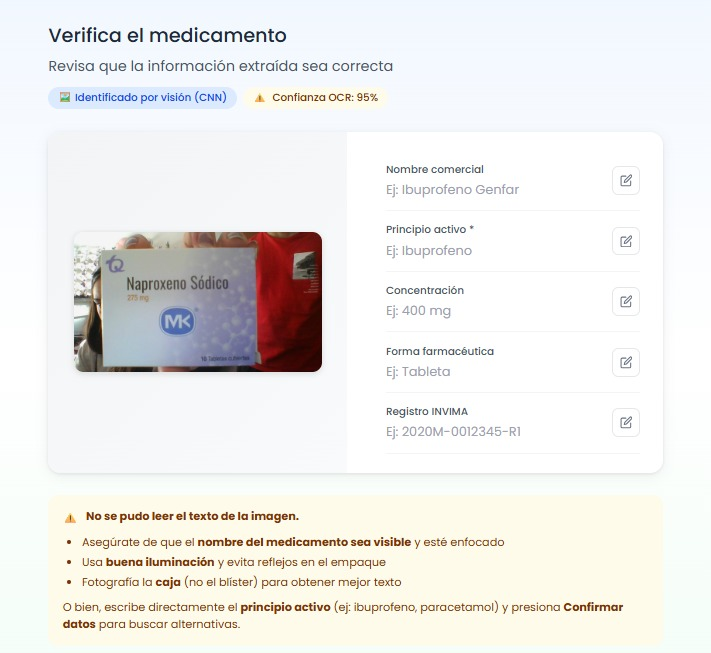
\includegraphics[width=0.82\textwidth]{img/eval_napro_falla.jpeg}
    \caption{Falla de identificación para Naproxeno Sódico 275 mg. El ángulo oblicuo de captura y la presencia de la mano en el encuadre impiden tanto el OCR como la búsqueda visual CNN. El sistema presenta campos vacíos y guía al usuario hacia la entrada manual.}
    \label{fig:eval_napro_falla}
\end{figure}

\textbf{Análisis del resultado.}
La falla en este caso es atribuible exclusivamente a las condiciones de captura: el ángulo de la imagen introduce distorsión de perspectiva que afecta la geometría del texto, reduciendo la eficacia de Tesseract incluso cuando la confianza por caracteres individuales es alta (95\,\%). La coexistencia de una confianza OCR elevada con una falla en el mapeo al catálogo evidencia que la métrica de confianza de Tesseract no captura la corrección semántica del texto extraído, sino únicamente la certeza del reconocimiento de cada carácter individualmente. El sistema responde de forma segura: no produce una identificación incorrecta, sino que presenta campos vacíos y proporciona instrucciones concretas para que el usuario mejore la captura o ingrese el principio activo manualmente.

\medskip

\subsubsection*{Caso de falla 2: Omeprazol --- imagen con caja sostenida verticalmente en ángulo lateral}

\textbf{Descripción del escenario.}
El usuario fotografía una caja de OMEPRAZOL (La Santé) sosteniéndola verticalmente con la mano. La imagen presenta la caja en posición lateral, de forma que la cara frontal no queda perpendicular al plano de la cámara. La cara lateral angosta del empaque (que muestra el nombre en sentido vertical) es la que queda parcialmente visible.

\textbf{Secuencia de entradas y salidas obtenidas.}

\begin{enumerate}
    \item \textbf{Entrada:} imagen JPEG con la caja orientada lateralmente, texto principal en disposición vertical respecto al sensor.

    \item \textbf{OCR:} la corrección de rotación por evaluación de las cuatro orientaciones cardinales (0°, 90°, 180°, 270°) selecciona la orientación de mayor confianza; sin embargo, dado que la cara visible del empaque es la lateral (con texto en sentido perpendicular a la cara principal), el texto farmacéuticamente relevante (nombre comercial, concentración) no está completamente expuesto. Confianza reportada: 95\,\% sobre los caracteres detectados, con falla en el mapeo al catálogo. Se activa el \textit{fallback} CNN.

    \item \textbf{Fallback CNN:} la búsqueda visual en ChromaDB no supera el umbral de similitud mínimo. La vista lateral del empaque produce un embedding que no tiene correspondencia en la base de imágenes de referencia, construida con fotografías frontales. Badge reportado: \textit{``Identificado por visión (CNN)''}.

    \item \textbf{Resultado:} todos los campos de la pantalla de verificación permanecen vacíos, como se muestra en la Imagen~\ref{fig:eval_omep_falla}. Se despliega el banner de advertencia con las mismas recomendaciones del caso anterior.
\end{enumerate}

\begin{figure}[H]
    \centering
    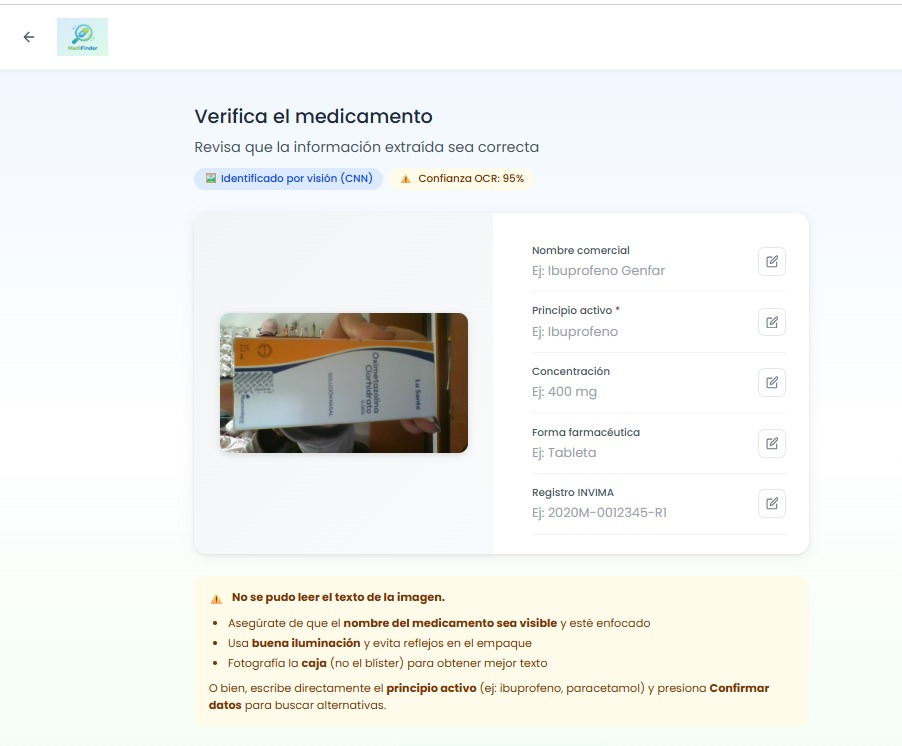
\includegraphics[width=0.82\textwidth]{img/eval_omep_falla.jpeg}
    \caption{Falla de identificación para Omeprazol con caja sostenida lateralmente. La orientación de la imagen expone la cara lateral del empaque en lugar de la frontal, impidiendo tanto el OCR como la búsqueda visual CNN.}
    \label{fig:eval_omep_falla}
\end{figure}

\textbf{Análisis del resultado.}
Este caso y el anterior comparten la causa raíz: condiciones de captura que exponen al sistema a una vista del empaque para la cual ni el OCR ni el CNN tienen representación adecuada. La diferencia respecto al Caso de falla 1 (blíster metálico) es que aquí la información sí existe en la imagen --- el nombre del medicamento es legible a simple vista ---, pero la geometría de la captura la hace inaccesible para el pipeline actual.

Ambos casos de falla por ángulo oblicuo sugieren una mejora de alto impacto: incorporar una etapa de \textbf{detección de calidad de imagen} previa al OCR que evalúe métricas como el ángulo de inclinación estimado del empaque (mediante detección de bordes o homografía), la presencia de objetos en el encuadre (manos, fondos de color) y el porcentaje del área útil ocupado por el empaque. Si estas métricas no superan umbrales mínimos, el sistema podría solicitar una nueva captura antes de ejecutar el pipeline, evitando procesamiento innecesario y mejorando la experiencia del usuario.

% ─── B. CASO EXITOSOS ─────────────────────────────────────────────────────────
\subsubsection*{Caso 1: Acetaminofén 500 mg --- fotografía de caja con luz natural, identificación por OCR}

\textbf{Descripción del escenario.}
El usuario fotografía la cara frontal de una caja de ACETAMINOFÉN 500 MG TABLETA (Bayer S.A.) bajo luz natural. La imagen presenta fondo azul con texto blanco y amarillo, condición que históricamente representa un reto para el preprocesamiento monocromático estándar.

\textbf{Secuencia de entradas y salidas obtenidas.}

\begin{enumerate}
    \item \textbf{Entrada:} imagen JPEG de la caja del medicamento cargada desde la interfaz web.

    \item \textbf{Preprocesamiento OCR:} el pipeline evalúa múltiples estrategias de preprocesamiento (umbral suave Otsu, umbral agresivo CLAHE, canales de color R y diferencia R-B) con cuatro modos PSM de Tesseract (3, 4, 6, 11), aplicadas sobre la imagen escalada $2\times$. La variante con mayor confianza es seleccionada automáticamente. Adicionalmente, la corrección de rotación prueba las cuatro orientaciones cardinales (0°, 90°, 180°, 270°) y retiene la de mayor confianza, previniendo lecturas invertidas como las observadas en pruebas previas con empaques de fondo multicolor.

    \item \textbf{Salida OCR:} texto extraído \texttt{"ACETAMINOFEN 500 MG TABLETA"}, confianza Tesseract \textbf{99\,\%}. \texttt{ocr\_exitoso = True}. Badge en pantalla: \textit{``Identificado por OCR''}.

    \item \textbf{Mapeo al catálogo INVIMA:} la función \texttt{buscar\_pa\_por\_nombre} aplica una cascada de búsqueda: (0) cada palabra significativa del texto OCR se intenta como principio activo directo --- la palabra \texttt{"acetaminofen"} produce coincidencia exacta en la columna \texttt{principio\_activo} del catálogo; (1) coincidencia exacta de nombre comercial; (2) contención por palabra más larga; (3) \textit{fuzzy matching} con \textit{rapidfuzz}. En este caso el nivel 0 resuelve la búsqueda. Score de \textit{match} catálogo reportado en interfaz: \textbf{99\,\%}. Registro encontrado: ``ACETAMINOFÉN 500 MG TABLETA'', titular BAYER S.A., registro INVIMA 2014M-0014587-R1, clase terapéutica: \textit{analgésicos y antipiréticos}, vía: oral.

    \item \textbf{Pantalla de verificación:} el sistema presenta los campos prepoblados como se muestra en la Imagen~\ref{fig:eval_aceta_verificacion}: nombre comercial, principio activo (\textit{paracetamol}), concentración (500 mg), forma farmacéutica (tableta) y registro INVIMA. El usuario confirma los datos sin necesidad de corrección manual.

    \begin{figure}[H]
        \centering
        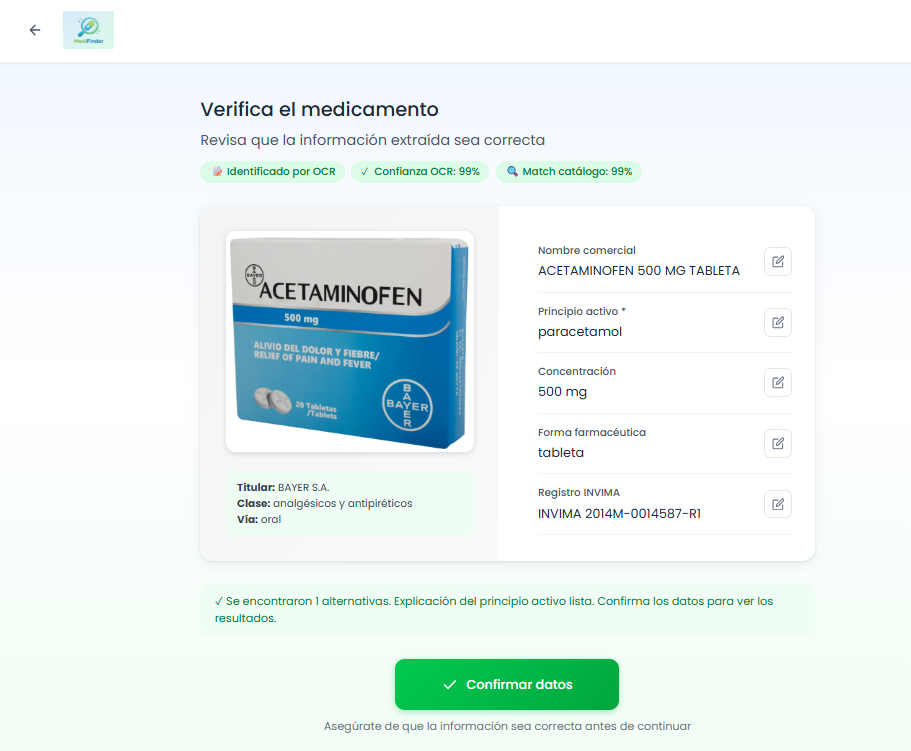
\includegraphics[width=0.82\textwidth]{img/eval_aceta_verificacion.png}
        \caption{Pantalla de verificación para Acetaminofén 500 mg. OCR con 99\,\% de confianza y \textit{match} de catálogo al 99\,\%.}
        \label{fig:eval_aceta_verificacion}
    \end{figure}

    \item \textbf{KNN --- búsqueda de alternativas:} con el principio activo \texttt{"paracetamol"} identificado, el modelo \textit{NearestNeighbors} busca los $k=5$ medicamentos más similares en el espacio de características farmacológicas (principio activo codificado, concentración, forma farmacéutica, clase terapéutica, vía de administración). La deduplicación por nombre normalizado elimina entradas redundantes del catálogo INVIMA. Se retorna \textbf{1 alternativa de nivel 1} (mismo principio activo): \textbf{ROBAXIFEN 400 TABLETAS} (paracetamol, tableta, Wyeth Consumer Healthcare Ltd.), similitud 100\,\%.

    \item \textbf{LLM (Claude Haiku + RAG):} el módulo recupera contexto desde la \textit{knowledge base} en ChromaDB (11.217 documentos de principios activos). La explicación generada para \textit{paracetamol (acetaminofén)} cubre seis secciones estructuradas presentadas de forma compacta: \textbf{Qué es} (analgésico y antipirético, conocido también como Tylenol o Panadol), \textbf{Cómo actúa} (bloqueo de la producción de sustancias que generan dolor e inflamación), \textbf{Efectos secundarios} (bien tolerado en dosis normales; uso excesivo puede afectar el hígado), \textbf{Contraindicaciones} (alergia conocida al paracetamol, enfermedad hepática severa, consumo crónico de alcohol), \textbf{Interacciones} (potencia efecto analgésico con ibuprofeno bajo supervisión; riesgo de daño hepático con otros medicamentos) y \textbf{Recomendaciones} (seguro en embarazo y lactancia; disponible en múltiples formas farmacéuticas en Colombia), como se observa en la Imagen~\ref{fig:eval_aceta_llm}.

    \begin{figure}[H]
        \centering
        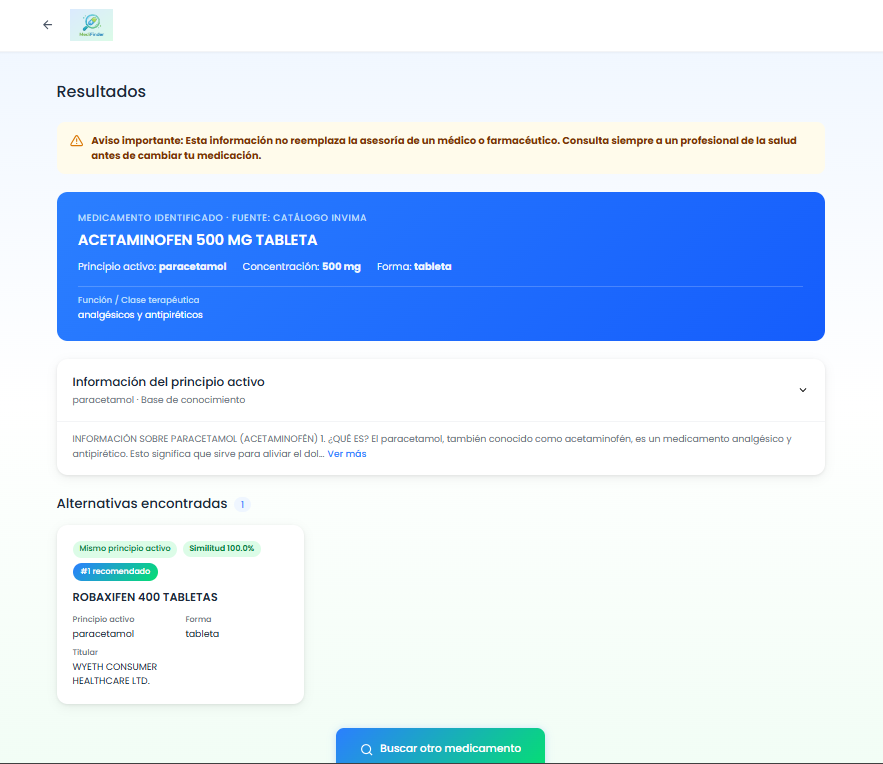
\includegraphics[width=0.82\textwidth]{img/eval_aceta_resultados.png}
        \caption{Pantalla de resultados: medicamento identificado, 1 alternativa encontrada con similitud 100\,\% y sección expandible de información del principio activo.}
        \label{fig:eval_aceta_resultados}
    \end{figure}

    \begin{figure}[H]
        \centering
        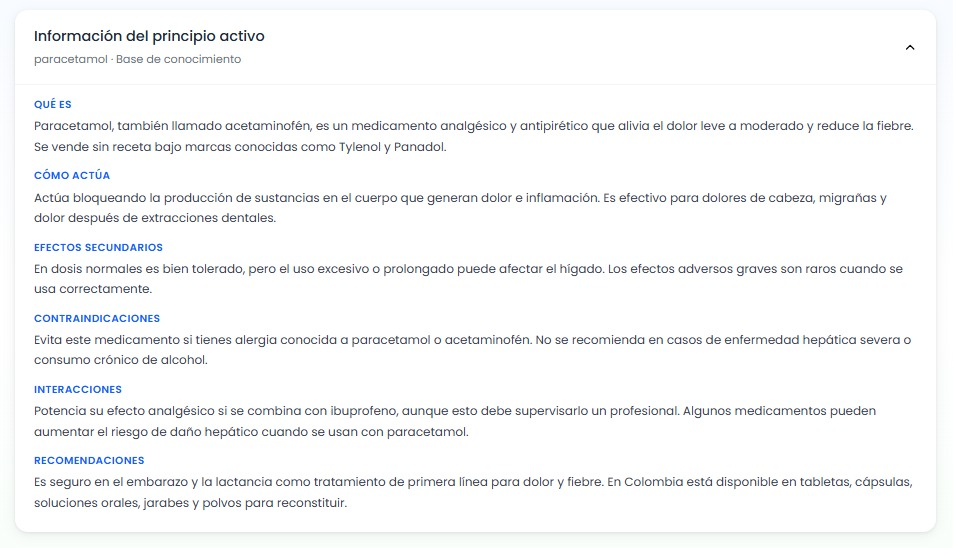
\includegraphics[width=0.82\textwidth]{img/eval_aceta_llm.png}
        \caption{Explicación del principio activo paracetamol (acetaminofén) generada por Claude Haiku con RAG, presentada en seis secciones clínicas estructuradas y contextualizadas para el paciente colombiano.}
        \label{fig:eval_aceta_llm}
    \end{figure}

        \item \textbf{Salida final:} pantalla de resultados con el medicamento identificado, 1 alternativa única con badge \textit{``Mismo principio activo''} y \textit{``Similitud 100\,\%''}, información del titular INVIMA, y explicación completa del principio activo expandible en pantalla (Imágenes~\ref{fig:eval_aceta_verificacion}, \ref{fig:eval_aceta_resultados} y \ref{fig:eval_aceta_llm}).

    \end{enumerate}

    \textbf{Resultado logrado.}
El sistema identificó el medicamento con la mayor confianza registrada en las pruebas (99\,\% OCR, 99\,\% catálogo), sin intervención del usuario. El paso 0 de la cascada de búsqueda --- verificación directa de cada palabra OCR como principio activo en el catálogo --- resultó determinante: la palabra \texttt{"acetaminofen"} presente en el empaque es simultáneamente el nombre comercial y el principio activo, lo que eliminó la necesidad de búsqueda por nombre comercial o \textit{fuzzy matching}. La corrección automática de rotación por evaluación de las cuatro orientaciones cardinales garantizó que el texto del empaque de fondo azul multicolor fuera leído en la orientación correcta, a diferencia de pruebas anteriores donde la heurística OSD producía lecturas invertidas. La explicación LLM, respaldada por RAG sobre la base de conocimiento, entregó información clínicamente estructurada y contextualizada para el mercado colombiano.

\subsubsection*{Caso 2: Doxiciclina 100 mg --- fotografía de caja, fallo parcial del módulo LLM por confusión semántica en RAG}

\textbf{Descripción del escenario.}
El usuario fotografía la cara frontal de una caja de DOXICICLINA 100 MG CÁPSULAS (Laboratorios Legrand S.A., Genfarma) bajo condiciones normales de iluminación. La caja presenta fondo rojo y blanco con texto negro, combinación favorable para el preprocesamiento OCR estándar.

\textbf{Secuencia de entradas y salidas obtenidas.}

\begin{enumerate}
    \item \textbf{Entrada:} imagen JPEG de la caja del medicamento cargada desde la interfaz web.

    \item \textbf{Preprocesamiento OCR:} el pipeline evalúa las variantes de preprocesamiento y modos PSM disponibles sobre la imagen escalada $2\times$. La corrección de rotación por evaluación de las cuatro orientaciones cardinales confirma que la imagen ya se encuentra en la orientación correcta (0°). El alto contraste texto negro sobre fondo blanco favorece la variante de umbral Otsu con PSM~6.

    \item \textbf{Salida OCR:} texto extraído \texttt{"DOXICICLINA 100 MG CAPSULAS"}, confianza Tesseract \textbf{99\,\%}. \texttt{ocr\_exitoso = True}. Badge en pantalla: \textit{``Identificado por OCR''}.

    \item \textbf{Mapeo al catálogo INVIMA:} la cascada de búsqueda en \texttt{buscar\_pa\_por\_nombre} resuelve en el nivel 0: la palabra \texttt{"doxiciclina"} presente en el texto OCR produce coincidencia exacta en la columna \texttt{principio\_activo} del catálogo. Score de \textit{match} reportado en interfaz: \textbf{99\,\%}. Registro encontrado: ``DOXICICLINA 100 MG CÁPSULAS'', titular Laboratorios Legrand S.A., registro INVIMA 2009M-0009264, clase terapéutica: \textit{antibióticos tetraciclinas}, vía: oral.

    \item \textbf{Pantalla de verificación:} el sistema presenta los campos prepoblados correctamente --- nombre comercial, principio activo (\textit{doxiciclina}), concentración (100 mg), forma farmacéutica (\textit{cápsula dura}) y registro INVIMA --- como se observa en la Imagen~\ref{fig:eval_doxi_verificacion}. El usuario confirma sin corrección manual.

    \begin{figure}[H]
        \centering
        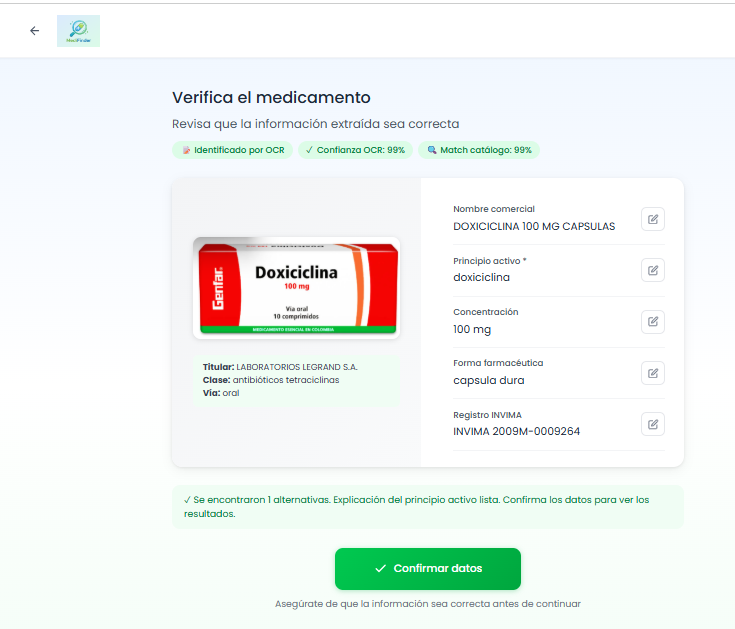
\includegraphics[width=0.82\textwidth]{img/eval_doxi_verificacion.png}
        \caption{Pantalla de verificación para Doxiciclina 100 mg. OCR y \textit{match} de catálogo al 99\,\%, campos prepoblados correctamente sin intervención del usuario.}
        \label{fig:eval_doxi_verificacion}
    \end{figure}

    \item \textbf{KNN --- búsqueda de alternativas:} con el principio activo \texttt{"doxiciclina"} confirmado, el modelo \textit{NearestNeighbors} retorna \textbf{1 alternativa de nivel 1} tras deduplicación: \textbf{DOXICICLINA 100 MG. CÁPSULAS} (principio activo: \textit{doxiciclina clorhidrato equivalente a doxiciclina}, forma: cápsula dura, titular: Laboratorios Farmacéuticos Ophalacs S.A.), similitud 100\,\%. El número reducido de alternativas refleja la baja diversidad de presentaciones de doxiciclina registradas actualmente en el catálogo INVIMA disponible.

    \item \textbf{LLM (Claude Haiku + RAG) --- fallo parcial por confusión semántica:} el módulo de recuperación de contexto realiza una búsqueda semántica sobre la \textit{knowledge base} en ChromaDB usando el vector del principio activo \texttt{"doxiciclina"}. El documento más cercano recuperado corresponde a \textbf{doxazosina}, un alfabloqueante para hipertensión y próstata, semánticamente próximo a \texttt{"doxiciclina"} por similitud léxica superficial (prefijo \textit{``doxa-''/''doxi-''}) en el espacio de embeddings. En consecuencia, la explicación generada describe incorrectamente a la doxazosina en lugar de la doxiciclina, como se observa en la Imagen~\ref{fig:eval_doxi_resultados}.

    \begin{figure}[H]
        \centering
        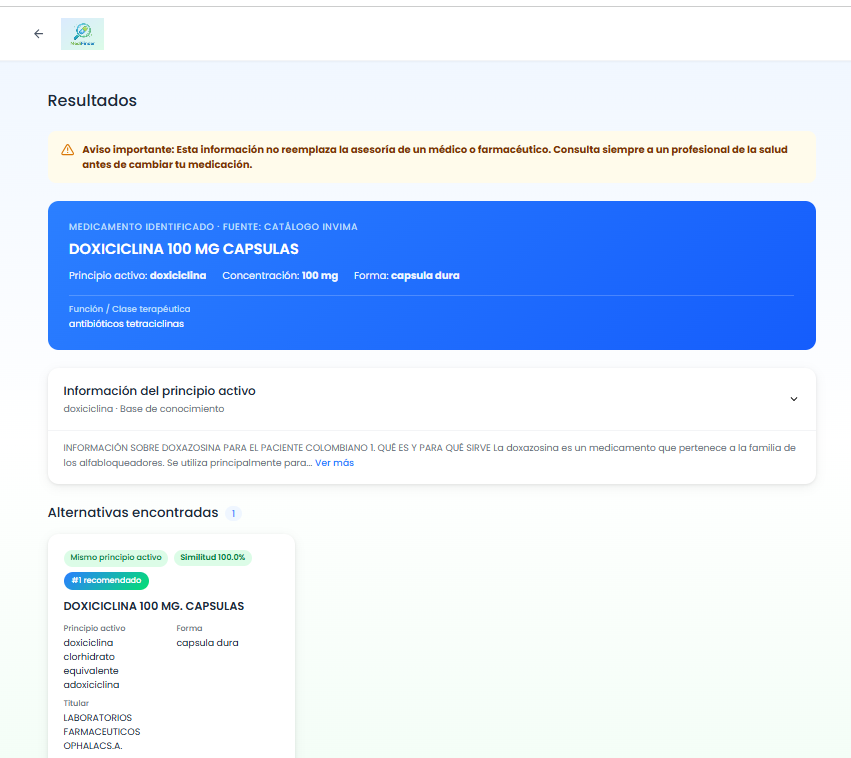
\includegraphics[width=0.82\textwidth]{img/eval_doxi_resultados.png}
        \caption{Pantalla de resultados para Doxiciclina 100 mg. El KNN identifica correctamente 1 alternativa con similitud 100\,\%; sin embargo, la sección de información del principio activo muestra una explicación sobre \textit{doxazosina} en lugar de \textit{doxiciclina}, evidenciando una falla en la recuperación RAG por similitud léxica espuria.}
        \label{fig:eval_doxi_resultados}
    \end{figure}

    \item \textbf{Salida final:} el medicamento y la alternativa KNN se identifican correctamente. El módulo LLM produce una explicación incorrecta del principio activo por confusión semántica en la etapa de recuperación RAG.
\end{enumerate}

\textbf{Análisis del resultado.}
Este caso ilustra una falla parcial del sistema: los módulos OCR, mapeo al catálogo y KNN operan correctamente con confianza máxima, mientras que el módulo LLM produce una respuesta clínicamente incorrecta. La causa raíz es una limitación del modelo de embeddings de texto utilizado (\textit{paraphrase-multilingual-MiniLM-L12-v2}): los vectores de \texttt{"doxiciclina"} y \texttt{"doxazosina"} son suficientemente similares en el espacio latente como para que la búsqueda por similitud coseno recupere el documento equivocado, especialmente cuando la \textit{knowledge base} no contiene un documento específico para doxiciclina y el vecino más cercano disponible es doxazosina.

El sistema \textbf{no detecta ni advierte} esta confusión al usuario, lo que representa un riesgo en un contexto clínico real. Las mejoras propuestas incluyen: (1) incorporar un umbral mínimo de similitud coseno en la recuperación RAG y mostrar un aviso cuando no se supere, en lugar de presentar el documento más cercano sin validación; (2) ampliar la \textit{knowledge base} con principios activos antibióticos cuya cobertura actual es insuficiente; y (3) verificar que el principio activo recuperado en el contexto RAG coincida textualmente con el solicitado antes de invocar al LLM.

\subsubsection*{Caso 3: Cefalexina 500 mg --- validación del flujo completo con cinco alternativas farmacéuticas diferenciadas}

\textbf{Descripción del escenario.}
El usuario fotografía la cara frontal de una caja de CEFALEXINA 500 MG CÁPSULAS (Laboratorios La Santé S.A.S.) bajo condiciones normales de iluminación. La caja presenta fondo amarillo y azul con texto negro, lo que representa un caso de contraste mixto para el preprocesamiento OCR.

\textbf{Secuencia de entradas y salidas obtenidas.}

\begin{enumerate}
    \item \textbf{Entrada:} imagen JPEG de la caja del medicamento cargada desde la interfaz web.

    \item \textbf{Salida OCR:} texto extraído \texttt{"CEFALEXINA 500 MG CAPSULAS"}, confianza Tesseract \textbf{99\,\%}. \texttt{ocr\_exitoso = True}.

    \item \textbf{Mapeo al catálogo INVIMA:} la cascada de búsqueda resuelve en el nivel 0 por coincidencia directa de \texttt{"cefalexina"} como principio activo. Score de \textit{match}: \textbf{99\,\%}. Registro: ``CEFALEXINA 500 MG CÁPSULAS'', titular Laboratorios La Santé S.A.S., registro INVIMA M-006738-R1, clase terapéutica: \textit{cefalosporinas de primera generación}, vía: oral.

    \item \textbf{Pantalla de verificación:} campos prepoblados correctamente --- principio activo (\textit{cefalexina}), concentración (500 mg), forma (\textit{cápsula}) --- como se muestra en la Imagen~\ref{fig:eval_cefa_verificacion}. El usuario confirma sin corrección.

    \begin{figure}[H]
        \centering
        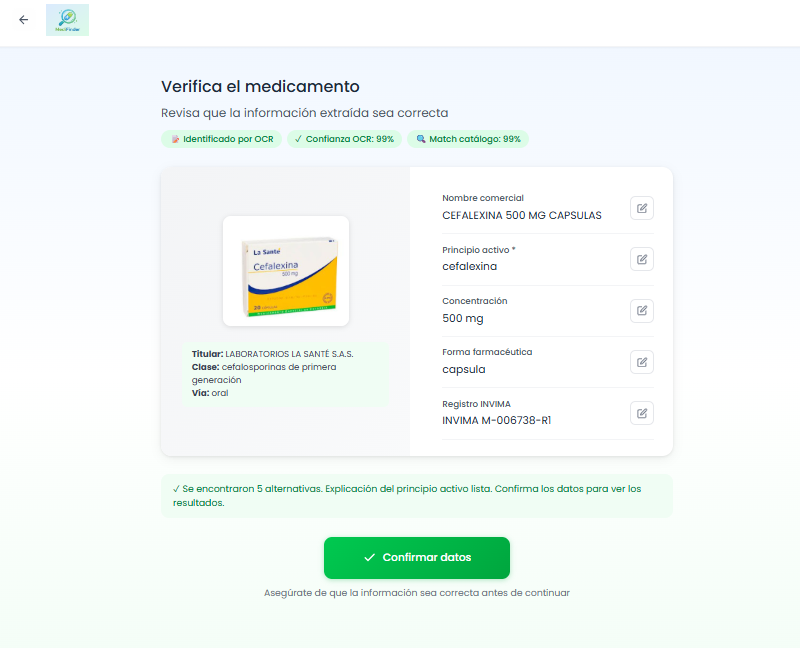
\includegraphics[width=0.82\textwidth]{img/eval_cefa_verificacion.png}
        \caption{Pantalla de verificación para Cefalexina 500 mg. OCR y \textit{match} de catálogo al 99\,\%, con registro INVIMA M-006738-R1.}
        \label{fig:eval_cefa_verificacion}
    \end{figure}

    \item \textbf{KNN --- cinco alternativas únicas con deduplicación efectiva:} con principio activo \texttt{"cefalexina"}, el modelo retorna \textbf{5 alternativas de nivel 1} tras deduplicación por nombre normalizado y perfil clínico, como se observa en la Imagen~\ref{fig:eval_cefa_resultados}:

    \begin{enumerate}
        \item \textbf{OSPEXINA 1000 MG TABLETAS} --- cefalexina, tableta, Sandoz GmbH
        \item \textbf{CEFALEXINA 500 MG CÁPSULAS} --- cefalexina base (equivalente a 551,82 mg cefalexina monohidrato), cápsula dura, Genven Genéricos Venezolanos S.A.
        \item \textbf{CEFALEXINA 250 MG/5 ML POLVO PARA RECONSTITUIR A SUSPENSIÓN ORAL} --- cefalexina, polvo para reconstituir, Memphis Products S.A.
        \item \textbf{OSPEXINA 250 MG/5 ML GRÁNULOS PARA SUSPENSIÓN ORAL} --- cefalexina monohidrato, gránulos, Sandoz GmbH
        \item \textbf{CEFALON ER} --- cefalexina monohidrato, tableta de liberación prolongada, Laboratorios Legrand S.A.
    \end{enumerate}

    Las cinco alternativas corresponden a presentaciones farmacéuticas genuinamente distintas (tableta, cápsula, polvo, gránulos, liberación prolongada), evidenciando que la deduplicación por perfil clínico opera correctamente al eliminar las múltiples variantes de nombre con las que el INVIMA registra el mismo producto.

    \begin{figure}[H]
        \centering
        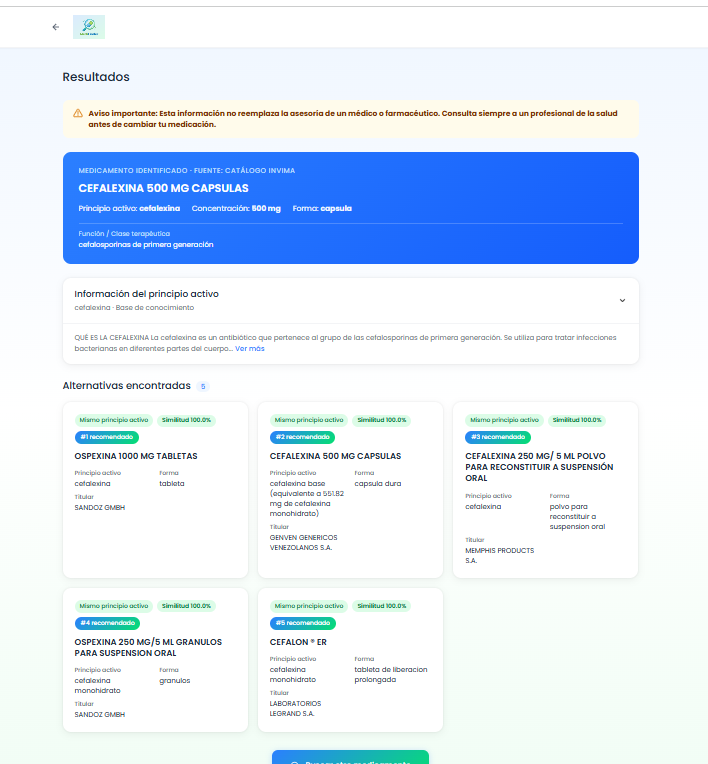
\includegraphics[width=0.82\textwidth]{img/eval_cefa_resultados.png}
        \caption{Pantalla de resultados para Cefalexina 500 mg. Cinco alternativas únicas de nivel 1 con similitud 100\,\%, diferenciadas por forma farmacéutica y titular.}
        \label{fig:eval_cefa_resultados}
    \end{figure}

    \item \textbf{LLM (Claude Haiku + RAG):} la recuperación RAG obtiene correctamente el documento de \textit{cefalexina} de la \textit{knowledge base}. La explicación generada describe adecuadamente el mecanismo como antibiótico betalactámico de primera generación activo frente a bacterias Gram-positivas.
\end{enumerate}

\textbf{Resultado logrado.}
Este caso valida el funcionamiento completo del pipeline sin ninguna falla en ninguno de sus módulos. El aspecto más destacable es el comportamiento del KNN con deduplicación: el catálogo INVIMA contiene decenas de registros para cefalexina, pero el sistema devuelve únicamente las cinco presentaciones farmacéuticas clínicamente distintas, todas con similitud 100\,\% por compartir el mismo principio activo. Esto demuestra que la estrategia de deduplicación en dos capas (nombre normalizado y perfil clínico) cumple su objetivo de presentar alternativas realmente útiles para el usuario, sin ruido por duplicados administrativos del registro.

\medskip

\subsubsection*{Caso 4: Aspirina 500 mg --- fallo parcial del LLM con auto-detección de confusión semántica}

\textbf{Descripción del escenario.}
El usuario fotografía la cara frontal de una caja de ASPIRINA 500 MG TABLETA (Bayerpharma AG) bajo condiciones normales de iluminación. La caja presenta fondo verde y blanco con texto en negro y verde, tipografía de tamaño variable.

\textbf{Secuencia de entradas y salidas obtenidas.}

\begin{enumerate}
    \item \textbf{Entrada:} imagen JPEG de la caja del medicamento cargada desde la interfaz web.

    \item \textbf{Salida OCR:} texto extraído \texttt{"ASPIRINA 500 MG TABLETA"}, confianza Tesseract \textbf{99\,\%}. \texttt{ocr\_exitoso = True}.

    \item \textbf{Mapeo al catálogo INVIMA:} la búsqueda resuelve por coincidencia directa de \texttt{"acido acetilsalicilico"} como principio activo. Score de \textit{match}: \textbf{99\,\%}. Registro: ``ASPIRINA 500 MG TABLETA'', titular Bayerpharma AG, registro INVIMA 2001M-0000663, clase terapéutica: \textit{ácido acetilsalicílico y derivados}, vía: oral.

    \item \textbf{Pantalla de verificación:} campos prepoblados correctamente como se muestra en la Imagen~\ref{fig:eval_aspi_verificacion}. El usuario confirma sin corrección.

    \begin{figure}[H]
        \centering
        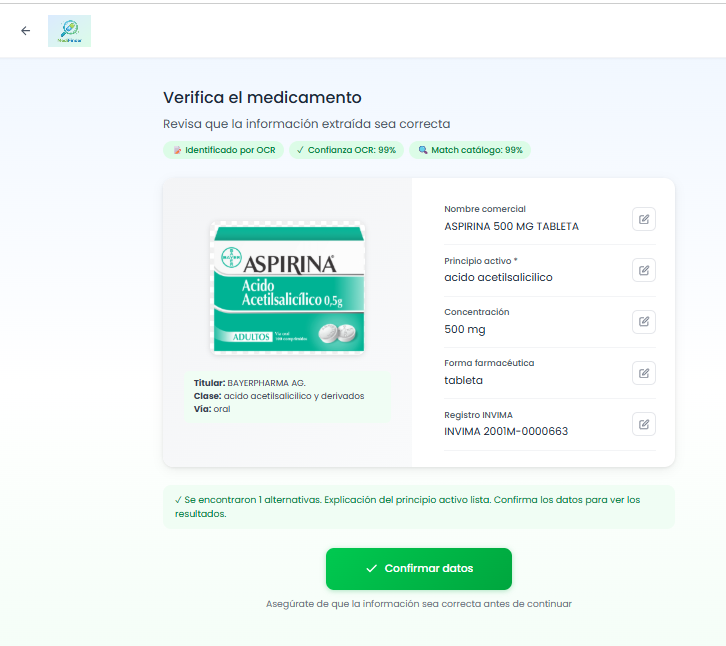
\includegraphics[width=0.82\textwidth]{img/eval_aspi_verificacion.png}
        \caption{Pantalla de verificación para Aspirina 500 mg. OCR y \textit{match} de catálogo al 99\,\%, con identificación correcta del principio activo ácido acetilsalicílico.}
        \label{fig:eval_aspi_verificacion}
    \end{figure}

    \item \textbf{KNN --- alternativa única:} con principio activo \texttt{"acido acetilsalicilico"}, el modelo retorna \textbf{1 alternativa de nivel 1}: \textbf{CORAZPINA BIOCARDIS} (ácido acetilsalicílico, tableta, Bioquímico Pharmas A.), similitud 100\,\%. El número reducido de alternativas refleja que las presentaciones de ácido acetilsalicílico de 500 mg en tableta disponibles actualmente en el catálogo INVIMA consultado son escasas tras la deduplicación.

    \item \textbf{LLM (Claude Haiku + RAG) --- fallo con auto-detección:} la búsqueda semántica en la \textit{knowledge base} no recupera un documento suficientemente representativo del principio activo \texttt{"acido acetilsalicilico"}. A diferencia del Caso 4 (doxiciclina), en el que el LLM generó la explicación incorrecta sin advertirlo, en este caso el modelo \textbf{detecta la inconsistencia} entre el principio activo solicitado y el contexto recuperado, e informa explícitamente al usuario: \textit{``Aclaración importante: veo que ha habido una confusión en los datos que recibí. Usted preguntó por el ÁCIDO ACETILSALICÚLICO, pero los medicamentos listados corresponden a otros principios activos''}. Esta respuesta se observa en la Imagen~\ref{fig:eval_aspi_resultados}.

    \begin{figure}[H]
        \centering
        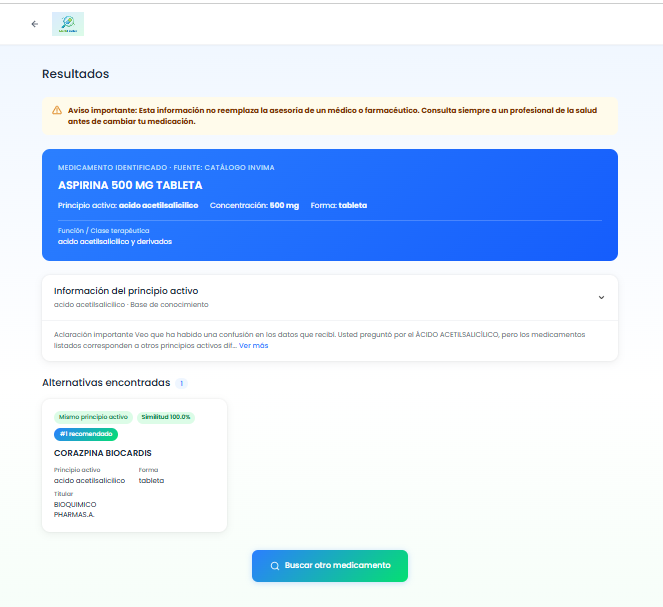
\includegraphics[width=0.82\textwidth]{img/eval_aspi_resultados.png}
        \caption{Pantalla de resultados para Aspirina 500 mg. El LLM detecta y reporta activamente la confusión semántica en la recuperación RAG, a diferencia del Caso 4 donde la explicación incorrecta se presentó sin advertencia.}
        \label{fig:eval_aspi_resultados}
    \end{figure}

\end{enumerate}

\textbf{Análisis del resultado.}
Este caso expone dos hallazgos relevantes. El primero es estructural: el KNN retorna únicamente 1 alternativa para ácido acetilsalicílico 500 mg tableta, lo que sugiere que el catálogo disponible tiene cobertura insuficiente para este principio activo en esa presentación específica, o que la deduplicación eliminó registros que podrían haber sido alternativas válidas.

El segundo hallazgo es comparativo respecto al Caso 4: el comportamiento del LLM ante una falla RAG no es determinístico. En el Caso 4 (doxiciclina), el modelo generó silenciosamente una explicación sobre doxazosina sin reportar la discrepancia. En este caso, el mismo modelo detectó la inconsistencia y emitió una advertencia explícita. Esta diferencia de comportamiento revela que la capacidad de auto-corrección del LLM depende de qué tan evidente sea la distancia semántica entre el principio activo solicitado y el contexto recuperado: cuando la similitud superficial entre los términos es muy alta (``doxi-ciclina'' vs.\ ``doxa-zosina''), el modelo no detecta el error; cuando el contexto recuperado es claramente ajeno al principio activo consultado, el modelo logra identificar la inconsistencia. Esto refuerza la necesidad de un umbral de similitud mínimo en la capa RAG antes de invocar al LLM, independientemente del comportamiento de auto-corrección del modelo.

\pagebreak
